\chapter*{Introduction}\label{ch:intro}

The importance of underwater cave mapping spans several fields. First, it is crucial in monitoring and tracking groundwater flows in karstic aquifers. According to Ford and Williams~\cite{Ford1994} 25\% of the world's population relays on karst water resources. Our work is motivated from the Woodville Karst Plain (WKP) which is a geomorphic region that extends from Central Leon County around the ``Big Bend'' of Florida~\cite{Lane2001}. Due to the significance of WKP, the Woodville Karst Plain Project (WKPP) has explored more than 34 miles of cave systems in Florida since 1987~\cite{WKPP}, proving the cave system to be the longest in USA~\cite{WKPP1}. This region is an important source of drinking water and is also a sensitive and vulnerable ecosystem. There is much to learn from studying the dynamics of the water flowing through these caves. Volumetric modeling of these caves will give researchers a better perspective about their size, structure, and connectivity. These models have even greater importance than simply enhancing the mapping. Understanding the volume of the conduits and how that volume increases and decreases over space is a critical component to characterizing the volume of flow through the conduit system. Current measurements are limited to point-flow velocities of the cave metering system and a cross-sectional volume at that particular point. My thesis work introduces a fist step towards robotic mapping of an underwater cave. The proposed approach results in 3\hyp D reconstructions which will give researchers the above described capabilities. Furthermore, volumetric models will be incredibly helpful for those involved with environmental and agricultural studies throughout the area, and once perfected this technology could help map other subterranean water systems, as well as any 3\hyp D environment that is difficult to map. The Woodville Karst Plain area is sensitive to seawater intrusions which threaten the agriculture and the availability of drinking water; for more details see the recent work by Zexuan et al.~\cite{ZexuanReports2016}. Second, detailed 3\hyp D representations of underwater caves will provide insights to the hydrogeological processes that formed the caves. Finally, because several cave systems contain historical records dating to the prehistoric times, producing accurate maps will be valuable to underwater archaeologists. 

\begin{figure}[ht]
	\begin{center}
		%\leavevmode
		\begin{tabular}{ccc}
			\hspace{-0.2em}\subfloat[]{\fbox{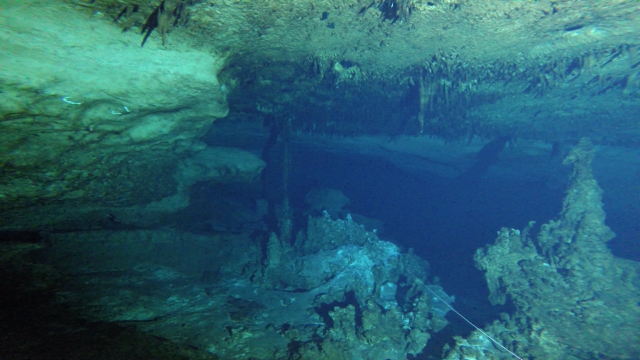
\includegraphics[width=.75\textwidth]{figures/Cave1S}\label{fig:beautyCave}}} \\
			\hspace{-0.5em}\subfloat[]{\fbox{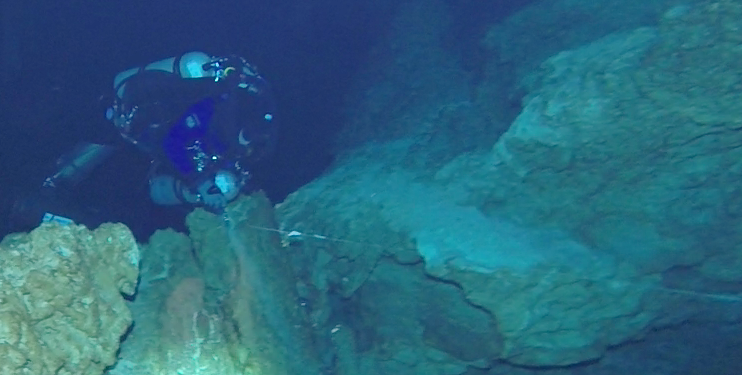
\includegraphics[width=.75\textwidth]{figures/DiverLine}\label{fig:diver}}}&
		\end{tabular}
	\end{center}
	\caption{\ref{fig:beautyCave} Typical Scene from an underwater cave. \ref{fig:diver} A cave diver attaching a branch line to the main line of a cave.}
	\label{fig:caveShots}
\end{figure}

Operations in underwater caves can be grouped under three categories: motion inside the known part of the cave; exploration of new territory; and surveying of newly explored areas. Most transportation in the explored part of caves is performed using diver propulsion vehicles (DPVs). All explored areas are marked by permanently attached cave line, which provides a direct route to the exit; see Fig. \ref{fig:diver} where a diver is inspecting the line. When divers explore uncharted territory, they proceed without the DPVs, laying out line and tying it to projections on the floor, walls, or ceiling. The third phase, surveying, consists of two divers measuring distances, using a cave\hyp line with knots every 3 m between attachment points. Simultaneously, the divers also measure the water depth at each attachment point, as well as the azimuth of the line leading to the next attachment point. All the information is recorded on a slate or waterproof paper. Estimates of the height and width of the passage can also be recorded, if time permits. The above described process is error\hyp prone and time consuming, and at greater depths results in significant decompression times, where total dive time can reach between 15 to 28 hours per dive. My thesis presents a first step of utilizing robotic technology to assist in cave exploration via the use of a stereo camera and a video\hyp light.  In many cases, during DPV rides, the divers attach cameras to their DPV and/or to themselves in order to document the exploration. Consequently, introducing a stereo camera does not complicate the standard operating procedures and will not increase the cognitive load of the divers.

The work of this thesis aims to achieve 3 goals.
\begin{enumerate}
	\item Study the implementation of camera calibration in a physical setting.
	\item Produce a point cloud of the underwater cave using stereo shape estimation and utilizing the presence of artificial light. 
	\item Reconstruct the surface of the cave out of the generated point cloud.
\end{enumerate} Combined, these pieces will come together to form a sufficient pipeline for reading image data and outputting a mapping of the cave system. This work can be easily adapted to a physical robot setting for later field use as described earlier. 

The next chapter will discuss a study of camera calibration along with effective methods for minimizing error in results. Chapter 3 covers the topic of scene reconstruction from stereo vision, and introduces a novel approach to generating point clouds of underwater cave systems\footnote{This chapter is joint work with Sharmin Rahman, Alberto Quattrini Li, and Ioannis Rekleitis and has appeared in the proceedings of the International Conference for Robotics and Automation (ICRA) 2017~\cite{weidner2017}.}. The last component, point cloud surface reconstruction, will be addressed in chapter 4. Finally, chapter 5 will conclude the work with a discussion of the overall contributions.